\ifdefined\handout
\documentclass[a4paper,handout]{beamer}
%\usepackage{auxtemplates}
\setbeamertemplate{footline}[frame number]
%\setbeamertemplate{footline}{\hfill\color{gray!90!blue} \insertframenumber/\inserttotalframenumber} 
%\usepackage{pgfpages}
%\pgfpagesuselayout{4 on 1}[a4paper]%,border shrink=5mm]
\else
\documentclass[a4paper]{beamer}
%\usepackage{beamerthemesplit}
\usetheme{Copenhagen}
%\usetheme{Warsaw}
\useoutertheme{shadow}
%\setbeamertemplate{footline}[frame plus slide number]
%\setbeamertemplate{footline}{\insertshortauthor \hfill \insertshorttitle \hfill \insertframenumber/\inserttotalframenumber}
\setbeamertemplate{footline}{
  \leavevmode%
  \hbox{
  \begin{beamercolorbox}[wd=.45\paperwidth,ht=2.5ex,dp=1.125ex,leftskip=.3cm plus1fill,rightskip=.3cm]{author in head/foot}%
    \usebeamerfont{author in head/foot}\insertshortauthor
  \end{beamercolorbox}%
  \begin{beamercolorbox}[wd=.40\paperwidth,ht=2.5ex,dp=1.125ex,leftskip=.3cm,rightskip=.3cm plus1fil]{title in head/foot}%
    \usebeamerfont{title in head/foot}\insertshorttitle
  \end{beamercolorbox}
  \begin{beamercolorbox}[wd=.1\paperwidth,ht=2.5ex,dp=1.25ex,leftskip=.3cm,rightskip =.3cm plus1fil]{page number}
   \insertframenumber/\inserttotalframenumber
  \end{beamercolorbox}
}%\vskip{0pt}
}

\setbeamertemplate{headline}
{%
  \leavevmode%
  \begin{beamercolorbox}[wd=\paperwidth,ht=2.5ex,dp=1.125ex]{section in head/foot}%
    \insertsectionnavigationhorizontal{\paperwidth}{\hskip0pt plus1filll}{}%
  \end{beamercolorbox}%
}

\fi
%%%%%%%%%%%%%%%%%%%%%%%%%%%%%%%%%%%%%%%%%%% Includes %%%%%%%%%%%%%%%%%%%%%%%%%%%%%%%%%%%%%%%%%%%%%%%%%%%%%%%%%
\usepackage{tkz-graph}


%%%%%%%%%%%%%%%%%%%%%%%%%%%%%%%%%%%%%%%%%%%%% Colors %%%%%%%%%%%%%%%%%%%%%%%%%%%%%%%%%%%%%%%%%%%%%%%%%%%%%%%%%
\colorlet{mygreen}{green!40!black}
\colorlet{myorange}{orange!80}
\colorlet{myblue}{blue!80!black}
\colorlet{myred}{red!60!black}
\newcommand{\red}[1]{\textcolor<2->{myred}{#1}}
\newcommand{\green}[1]{\textcolor<2->{mygreen}{#1}}

%%%%%%%%%%%%%%%%%%%%%%%%%%%%%%%%%%%%%%%%%% Definitions %%%%%%%%%%%%%%%%%%%%%%%%%%%%%%%%%%%%%%%%%%%%%%%%%%%%%%%
\newcommand{\pname}[1]{\textsc{#1}}
\newcommand{\ccsp}{\#CSP}
\newcommand{\cccsp}{\#CSP\(_c\)}
\newcommand{\cbis}{\#\textsc{BIS}}
\newcommand{\chom}{\#Hom}
\newcommand{\cdsp}{\pname{\#DownSets}}
\newcommand{\cp}{\#P}
\newcommand{\npc}{NP-complete}
\newcommand{\npC}{NP-Complete}
\newcommand{\cpC}{\#P-Complete}
\newcommand{\cpc}{\#P-complete}
\newcommand{\csat}{\#SAT}
\newcommand{\dsat}{2-SAT}
\newcommand{\tsat}{3-SAT}
\newcommand{\ctsat}{\#3-SAT}
\newcommand{\cdsat}{\#2-SAT}
\newcommand{\tcoloring}{\pname{3-Coloring}}
\newcommand{\ctcol}{\pname{\#3-Coloring}}
\newcommand{\cdcol}{\pname{\#2-Coloring}}
\newcommand{\cisp}{\#IS}
\newcommand{\cis}{\#\mathrm{IS}}
\newcommand{\cds}{\#\mathrm{DS}}
\newcommand{\impl}{\mathcal{P}}
\newcommand{\aple}{\le_{AP}}
\newcommand{\apge}{\ge_{AP}}
\newcommand{\apeq}{\equiv_{AP}}
\newcommand{\maple}{\(\aple\)}
\newcommand{\mapge}{\(\apge\)}
\newcommand{\setof}[1]{\{{#1}\}}
\newcommand{\oneto}[1]{{1,2,\dotsc,#1}}
\newcommand{\zto}[1]{{0,1,\dotsc,#1}}
\newcommand{\zo}{{0,1}}
\newcommand{\oneoeps}{\frac{1}{\epsilon}}
\newcommand{\oneoepsp}{\frac{1}{\epsilon'}}
\newcommand{\eps}{\epsilon}

\theoremstyle{definition}
\newtheorem{conj}{Conjecture}
%%%%%%%%%%%%%%%%%%%%%%%%%%%%%%%%%%%%%%%% Title Info %%%%%%%%%%%%%%%%%%%%%%%%%%%%%%%%%%%%%%%%%%%%%%%%%%%%%%%%%%
\author{Amir Hedayaty}
\title{Complexity of Approximating \#CSPs}
\institute{Simon Fraser University}
\date{Oct 30th 2012}

%%%%%%%%%%%%%%%%%%%%%%%%%%%%%%%%%%%%%%%%% Begin %%%%%%%%%%%%%%%%%%%%%%%%%%%%%%%%%%%%%%%%%%%%%%%%%%%%%%%%%%%%%%%%%
\begin{document}
\begin{frame}
\titlepage
\end{frame}

\begin{frame}
\frametitle{Table of Contents}
\tableofcontents
\end{frame}

%%%%%%%%%%%%%%%%%%%%%%%%%%%%%%%%%%%%%%%%%%%%%%%%%%%%%%%%%%%%%%%%%%%%%%%%%%%%%%%%%%%%%%%%%%%%%%%%%%%%%%%%%%%%%%%%%%%%%
\section{Introduction}
%%%%%%%%%%%%%%%%%%%%%%%%%%%%%%%%%%%%%%%%%%%%%%%%%%%%%%%%%%%%%%%%%%%%%%%%%%%%%%%%%%%%%%%%%%%%%%%%%%%%%%%%%%%%%%%%%%%%%

\begin{frame}
\frametitle{CSP}
A \textcolor{mygreen}{constraint language} \(\Gamma\) is a set of relations
\pause \onslide<3->{\(\Gamma = \{R_1,R_2\}\)}
\vskip 12pt
A CSP(\(\Gamma\)) instance \(\mathcal{P} = (D, V, \mathcal{C})\)
\begin{itemize}
\item \(D\) is a domain \onslide<3-> {\(\{1,2,3\}\)}
\item \(V\) is a set of variables \onslide<3-> {\(\{x_1,x_2,x_3,x_4\}\)}
\item \(\mathcal{C}\) is a set of constraints \\
\onslide<3-> {\(\{\langle R_1, (x_1,x_2)\rangle, \langle R_2, (x_1, x_4, x_3)\rangle, \langle R_1, (x_2,x_4) \rangle \)\}}
\end{itemize}
\vskip 12pt
\pause % for <2->
\vskip 12pt

\pause
A solution \(\varphi\) for \(\mathcal{P}\) is an assignment of \(V\) to \(D\) satisfying all the constraints in \(\mathcal{C}\)
\pause
\begin{eqnarray*}
&&\varphi(x_1)=1, \varphi(x_2)=3, \varphi(x_3)=1, \varphi(x_4)=2 \\
&&(1,3) \in R_1, (1,2,2) \in R_2, (3,2) \in R_1
\end{eqnarray*}
\end{frame}

%%%%%%%%%%%%%%%%%%%%%%%%%%%%%%%%%%%%%%%
\begin{frame}
\frametitle{The Problem CSP(\(\Gamma\))}
\begin{definition} [The Problem CSP(\(\Gamma\))]
Input: an instance \(\mathcal{P}\) with constraint language \(\Gamma\) \\
Decide if \(\mathcal{P}\) has a solution
\end{definition}
\begin{conj} [Feder and Vardi 1998]
The problem CSP(\(\Gamma\)) is either polynomial time solvable or NP-complete
\end{conj}
\end{frame}

%%%%%%%%%%%%%%%%%%%%%%%%%%%%%%%%%%%%%%%
\begin{frame}
\frametitle{\tcoloring}
The problem \tcoloring\ can be expressed with CSP(\(\Gamma\))
\pause
\begin{eqnarray*}
&&D=\{r,g,b\}\\
&&R=\{(r,g),(r,b),(g,r),(g,b),(b,r), (b,g)\}\\
&&x\sim y \Rightarrow \langle R, (x,y)\rangle \in \mathcal{C} \
\end{eqnarray*}
\end{frame}

%%%%%%%%%%%%%%%%%%%%%%%%%%%%%%%%%%%%%%%
\begin{frame}
\frametitle{\tsat}
\onslide<1->{The problem \tsat\ can be expressed with CSP(\(\Gamma\))}
\pause
\begin{eqnarray*}
&&D=\{T,F\}\\
&&\Gamma = \{R_1, R_2, R_3, R_4, R_5, R_6, R_7, R_8\}\\
&&R_1=\{(x,y,z)\mid x,y,z\in \setof{T,F}, x \lor y \lor z = T\}\\
&&R_2=\{(x,y,z)\mid x,y,z\in \setof{T,F}, \bar x \lor y \lor z = T\}\\
&&R_3=\{(x,y,z)\mid x,y,z\in \setof{T,F}, x \lor \bar y \lor z = T\}\\
&&R_4=\{(x,y,z)\mid x,y,z\in \setof{T,F}, x \lor y \lor \bar z = T\}\\
&&R_5=\{(x,y,z)\mid x,y,z\in \setof{T,F}, \bar x \lor \bar y \lor z = T\}\\
&&R_6=\{(x,y,z)\mid x,y,z\in \setof{T,F}, \bar x \lor y \lor \bar z = T\}\\
&&R_7=\{(x,y,z)\mid x,y,z\in \setof{T,F}, x \lor \bar y \lor \bar z = T\}\\
&&R_8=\{(x,y,z)\mid x,y,z\in \setof{T,F}, \bar x \lor \bar y \lor \bar z = T\}
\end{eqnarray*}
\pause
Note that \(\Gamma' = \{R_1, R_2, R_5, R_8\}\) is sufficient for \tsat
\end{frame}

%%%%%%%%%%%%%%%%%%%%%%%%%%%%%%%%%%%%%%%
\begin{frame}
\frametitle{Graph Homomorphism}
\begin{definition} [Homomorphism]
A homomorphism is mapping from \(V(G) \to V(H)\) such that
\[x\sim y \Rightarrow h(x)\sim h(y)\]
\end{definition}
\pause
\begin{center}
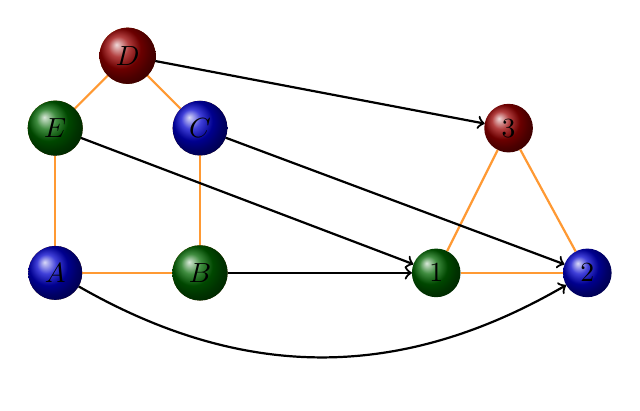
\begin{tikzpicture}
\GraphInit[vstyle=Shade]
\SetVertexMath
\tikzset{VertexStyle/.style ={shape=circle,ball color = myorange,}}
\begin{scope}[rotate=-135]
\Vertices[unit=1.3]{circle}{A,B,C,E}
\end{scope}
\NOEA[unit=.919](E){D}
\tikzset{EdgeStyle/.style = {color=myorange}}
\Edges(A,B,C,D,E,A)
\tikzset{VertexStyle/.style ={shape=circle,ball color = mygreen,}}
\EA[unit=3](B) {1}
\tikzset{VertexStyle/.style ={shape=circle,ball color = myblue,}}
\EA[unit=4.919](B) {2}
\tikzset{VertexStyle/.style ={shape=circle,ball color = myred,}}
\EA[unit=3.919](C) {3}
\Edges(1,2,3,1)
\onslide<3->{
\tikzset{EdgeStyle/.style = {->, bend right}}
\Edge (A)(2)
%\tikzset{EdgeStyle/.style = {->, bend left}}
\tikzset{EdgeStyle/.style = {->}}
\Edge (B)(1)
\Edge (E)(1)
\Edge (D)(3)
\Edge (C)(2)
\tikzset{VertexStyle/.style={shape=circle, ball color = myred,}}
\Vertex[Node]{D}
\tikzset{VertexStyle/.style={shape=circle, ball color = myblue,}}
\Vertex[Node]{A}
\Vertex[Node]{C}
\tikzset{VertexStyle/.style={shape=circle, ball color = mygreen,}}
\Vertex[Node]{B}
\Vertex[Node]{E}
}
\end{tikzpicture}
\end{center}
\pause
\end{frame}

%%%%%%%%%%%%%%%%%%%%%%%%%%%%%%%%%%%%%%%
\begin{frame}
\frametitle{CSP and homomorphism}
CSP generalizes graph homomorphism
\pause

Any homomorphism \(h\) from \(G=(V_G, E_G)\) to \(H=(V_H, E_H)\) \\
corresponds to \\
a solution \(\varphi\) in \(\mathcal{P}=(D,V,\mathcal{C})\) of CSP(\(\Gamma\))
\begin{itemize}
\item \(D = V_H\)
\item \(V = V_G\)
\item \(\Gamma \gets E_H\)
\item \(\mathcal{C} \gets E_G \)
\end{itemize}
\end{frame}

%%%%%%%%%%%%%%%%%%%%%%%%%%%%%%%%%%%%%%%
\begin{frame}
\frametitle{The Problem Hom(\(H\))}
\begin{definition} [The problem Hom(\(H\))]
Input: a graph \(G\)\\
Decide if there exists a homomorphism from \(G\) to \(H\)
\end{definition}

\begin{theorem} [Hell and Ne\v{s}et\v{r}il 1990]
Let \(H\) be a graph\\
If \(H\) is bipartite or has a loop, Hom(\(H\)) is polynomial time solvable\\
Otherwise Hom(\(H\)) is NP-complete
\end{theorem}
\end{frame}

%%%%%%%%%%%%%%%%%%%%%%%%%%%%%%%%%%%%%%%
\begin{frame}
\frametitle{\ccsp(\(\Gamma\))}
\begin{definition} [The Problem \ccsp(\(\Gamma\))]
Input: an instance \(\mathcal{P}\) with constraint language \(\Gamma\) \\
The number of solutions for \(\mathcal{P}\)
\end{definition}

The problems \ctcol\ and \ctsat\ can be expresses by \ccsp(\(\Gamma\))
\begin{definition} [The problem \chom(\(H\))]
Input: a graph \(G\)\\
The number of homomorphisms from \(G\) to \(H\)
\end{definition}
\end{frame}

%%%%%%%%%%%%%%%%%%%%%%%%%%%%%%%%%%%%%%%
\begin{frame}
\frametitle{FP and \cp}
\begin{definition} [FP]
The set of functions computable in polynomial time using deterministic Turing machine
\end{definition}

\begin{definition}[\cp]
The set of functions expressible by the number of accepting paths of a polynomial time non-deterministic Turing machine
\end{definition}
\end{frame}

%%%%%%%%%%%%%%%%%%%%%%%%%%%%%%%%%%%%%%%%%%%%%%%%%%%%%%%%%%%%%%%%%%%%%%%%%%%%%%%%%%%%%%%%%%%%%%%%%%%%%%%%%%%%%%%%%%%%%
\section{Background}
%%%%%%%%%%%%%%%%%%%%%%%%%%%%%%%%%%%%%%%%%%%%%%%%%%%%%%%%%%%%%%%%%%%%%%%%%%%%%%%%%%%%%%%%%%%%%%%%%%%%%%%%%%%%%%%%%%%%%

%%%%%%%%%%%%%%%%%%%%%%%%%%%%%%%%%%%%%%%
\begin{frame}
\frametitle{Major Results on \ccsp}
\begin{theorem} [Creignou and Hermann 1996]
Let \(\Gamma\) be a Boolean constraint language\\
If \(\Gamma\) is affine, \ccsp(\(\Gamma\)) is polynomial time solvable\\
Otherwise \ccsp(\(\Gamma\)) is \cpc
\end{theorem}

\pause

\begin{theorem} [Dyer and Greenhill 2000] 
Let \(H\) be a graph\\
If each connected component of \(H\) is 
\begin{itemize}
\item a complete reflexive graph
\item a complete irreflexive bipartite graph
\end{itemize}
\chom(\(H\)) is polynomial time solvable\\
Otherwise \chom(\(H\)) is \cpc
\end{theorem}
\end{frame}

%%%%%%%%%%%%%%%%%%%%%%%%%%%%%%%%%%%%%%%
\begin{frame}
\frametitle{Major Results on \ccsp\ Continued}
\begin{theorem} [Bulatov 2008]
\ccsp(\(\Gamma\)) is either polynomial time solvable or \cpc
\end{theorem}
\pause

\begin{theorem}[Dyer and Richerby 2010]
Bulatov's dichotomy property is in NP.
\end{theorem}
\end{frame}

%%%%%%%%%%%%%%%%%%%%%%%%%%%%%%%%%%%%%%%
\begin{frame}
\frametitle{FPRAS}
FPRAS is the efficient model for approximation
\begin{block} {\(f \in \) FPRAS}
There exists an algorithm \\
Input: \(x\), \(\eps\) \\
Output: \(y\) such that with probability \( > \frac{3}{4}\)
\[\left|\frac{y-f(x)}{f(x)}\right| \le \eps\]
Running time: polynomial in terms of \(|x|\) and \(\oneoeps\)
\end{block}
\end{frame}

%%%%%%%%%%%%%%%%%%%%%%%%%%%%%%%%%%%%%%%
\begin{frame}
\frametitle{APX}
APX schemes are algorithms with approximation ratio \(\alpha\) \\
\vskip 12pt
\pause
\begin{theorem}
If there is an \(\alpha\)-APX for \ccsp(\(\Gamma\)), there an FPRAS for \ccsp(\(\Gamma\))
\end{theorem}
\vskip 12pt
APX schemes are not used for \ccsp(\(\Gamma\))
\end{frame}

%%%%%%%%%%%%%%%%%%%%%%%%%%%%%%%%%%%%%%%
\begin{frame}
\frametitle{Approximation Preserving Reductions}
\begin{definition}[AP-reduction]
if \(f \aple g\) \\
\[g \in FPRAS \Rightarrow f \in FPRAS\]
\end{definition}

\pause
If \(f \aple g\) and \(g \aple f\) then \(f \apeq g\) or \\
\(f\) and \(g\) are \textcolor{mygreen}{AP-interreducible}
\end{frame}

%%%%%%%%%%%%%%%%%%%%%%%%%%%%%%%%%%%%%%%
\begin{frame}
\frametitle{Polynomial time Solvable}
\begin{center}
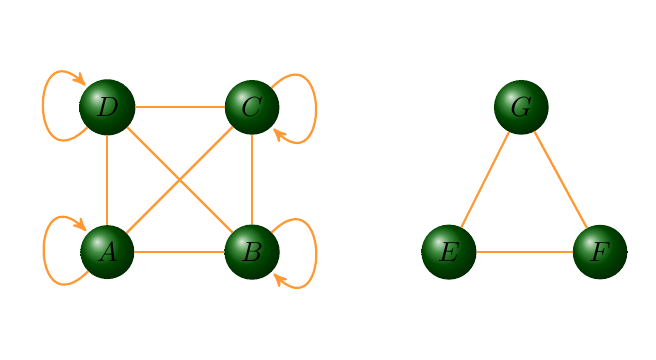
\begin{tikzpicture}
\GraphInit[vstyle=Shade]
\SetVertexMath
\tikzset{EdgeStyle/.style ={color = myorange}}
\tikzset{VertexStyle/.style ={shape=circle,ball color = mygreen,}}
\begin{scope}[rotate=-135]
\Vertices[unit=1.3]{circle}{A,B,C,D}
\end{scope}
\Edges(A,B,C,D,A)
\Edge (A)(C)
\Edge (B)(D)
\Loop[dist=30pt, dir=WE](A)
\Loop[dist=30pt, dir=EA](B)
\Loop[dist=30pt, dir=EA](C)
\Loop[dist=30pt, dir=WE](D)
\EA[unit=2.5](B) {E}
\EA[unit=4.419](B) {F}
\EA[unit=3.419](C) {G}
\Edges(E,F,G,E)
\end{tikzpicture}
\end{center}

\pause
Problems \pname{\#Dual-SAT} and \pname{\#Match} are also in FPRAS
\end{frame}

%%%%%%%%%%%%%%%%%%%%%%%%%%%%%%%%%%%%%%%
\begin{frame}
\frametitle{Problems Hard to Approximate}
These problems are \\
\cpc\ with respect to AP-reduction \\
\begin{center}
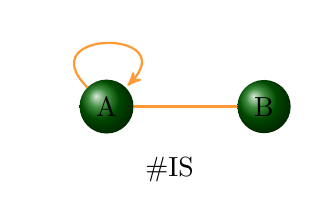
\begin{tikzpicture}
\GraphInit[vstyle=Shade]
\node[inner sep=0,anchor=east,text width=2cm] (note1) at (2.5,-.8) {\cisp};
\tikzset{EdgeStyle/.style ={color = myorange}}
\tikzset{VertexStyle/.style ={shape=circle,ball color = mygreen,}}
\Vertices[unit=2]{line}{A,B}
\Edge (A)(B)
\Loop[dist=30pt, dir=NO](A)
\end{tikzpicture}
\end{center}
\vskip 12pt
\pause
The problems \csat, \ctsat, and \cdsat\ are also in this family
\end{frame}

%%%%%%%%%%%%%%%%%%%%%%%%%%%%%%%%%%%%%%%
\begin{frame}
\frametitle{\cbis}
\begin{center}
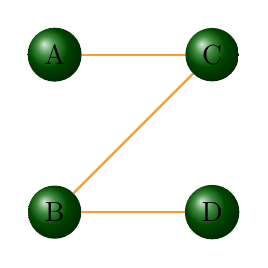
\begin{tikzpicture}
\GraphInit[vstyle=Shade]
\tikzset{EdgeStyle/.style ={color = myorange}}
\tikzset{VertexStyle/.style ={shape=circle,ball color = mygreen,}}
\Vertex[x=0, y=2] {A}
\Vertex[x=0, y=0] {B}
\Vertex[x=2, y=2] {C}
\Vertex[x=2, y=0] {D}
\Edges (A,C,B,D)
\end{tikzpicture}
\end{center}

\begin{definition}[\cbis]
Input: A bipartite graph \(G\)\\
Output: The number of independent sets in \(G\)
\end{definition}
\end{frame}

%%%%%%%%%%%%%%%%%%%%%%%%%%%%%%%%%%%%%%%
\begin{frame}
\frametitle{\cdsp}
\begin{center}
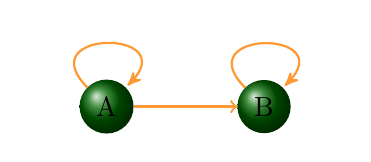
\begin{tikzpicture}
\GraphInit[vstyle=Shade]
\tikzset{EdgeStyle/.style ={->, color = myorange}}
\tikzset{VertexStyle/.style ={shape=circle,ball color = mygreen,}}
\Vertices[unit=1]{circle}{B,A}
\Edge (A)(B)
\Loop[dist=30pt, dir=NO](A)
\Loop[dist=30pt, dir=NO](B)
\end{tikzpicture}
\end{center}

\begin{definition} [\cdsp]
Input: A partial order \(P\) \\
Output: The number of downsets in \(P\)
\end{definition}
\end{frame}

%%%%%%%%%%%%%%%%%%%%%%%%%%%%%%%%%%%%%%%
\begin{frame}
\frametitle{Trichotomy}
\begin{theorem} [Dyer, Goldberg and Jerrum 2010]
Let \(\Gamma\) be a Boolean constraint language\\
\begin{itemize}
\item if \(\Gamma\) is affine, \ccsp(\(\Gamma\)) is polynomial time solvable
\item otherwise if \(\Gamma\) is monotone, \ccsp(\(\Gamma\)) is AP-interreducible with \cbis
\item otherwise \ccsp(\(\Gamma\)) is \cpc\ with respect to AP-reductions
\end{itemize}
\end{theorem}
\end{frame}

%%%%%%%%%%%%%%%%%%%%%%%%%%%%%%%%%%%%%%%
\begin{frame}
\frametitle{Techniques For AP-reductions}
Let \(A\) and \(B\) be two counting problems; \(B \aple A\) if
\begin{itemize}
\item \(B\) is same as \(A\) only the input is connected\\
\pause
\item both \(A\) and \(B\) have always at least one solution\\
there is a function \(\varphi\) mapping an instance \(\mathcal{P}\) of \(B\) to an instance of \(A\) such that
\[\#\mathcal{P} = a \cdot \#\varphi(\mathcal{P}) + b\]
\end{itemize}
\end{frame}

%%%%%%%%%%%%%%%%%%%%%%%%%%%%%%%%%%%%%%%
\begin{frame}
\frametitle{Pinning}
Pinning is the ability to tie a variable to a certain set of values
\vskip 12pt
\pause
Let \(\Gamma\) be a constraint language over \(D\)\\
Let \(R \in \Gamma\) and \(S \subseteq D\) 
\pause
\begin{lemma}
If \(S\) is the set of reflexive vertices in \(R\)
\[\mathrm{\ccsp(}\Gamma \cup \{S\}\mathrm{)} \aple \mathrm{\ccsp(}\Gamma\mathrm{)}\]
\end{lemma}
\begin{lemma}[Extended Pinning]
if for some \(j\), for all \(a \in S\) TODO
\[\mathrm{\ccsp(}\Gamma \cup \{S\}\mathrm{)} \aple \mathrm{\ccsp(}\Gamma\mathrm{)}\]
\end{lemma}
\end{frame}


%%%%%%%%%%%%%%%%%%%%%%%%%%%%%%%%%%%%%%%
\begin{frame}
\frametitle{Maximization}
Let \(\mathcal{P} = (\{1,2,3\}, \{x_1,x_2,y_1,y_2,y_3\}, \mathcal{C})\) be an instance of CSP(\(\Gamma\))\\
The number of solutions grouped by \(x_1, x_2\) are as follows
\begin{eqnarray*}
\begin{array}{c|ccccccccc}
x_1 & \green{1} & \green{1} & \green{1} & 2 & \green{2} & \green{2} & 3 & 3 & \green{3}\\
x_2 & \green{1} & \green{2} & \green{3} & 1 & \green{2} & \green{3} & 1 & 2 & \green{3}\\
\hline
\#  & \red{7} & \red{7} & \red{7} & 5 & \red{7} & \red{7} & 4 & 3 & \red{7}\\ 
\end{array}
\end{eqnarray*}
\pause
\(7\) is the maximum number here \\
\pause
\(\mathcal{P}\) is a \textcolor{mygreen}{max-implementation} of \(R\) by \(\Gamma\)
\[R = \{(1, 1), (1, 2), (1, 3), (2, 2), (2, 3), (3,3)\}\]
\end{frame}

%%%%%%%%%%%%%%%%%%%%%%%%%%%%%%%%%%%%%%%
\begin{frame}
\frametitle{Maximization Theorem}
\begin{theorem}
If \(\Gamma\) max-implements \(R\)
\[\mathrm{\#CSP(}\Gamma \cup \{R\}\mathrm{)} \aple \mathrm{\#CSP(}\Gamma\mathrm{)}\]
\end{theorem}
\end{frame}

%%%%%%%%%%%%%%%%%%%%%%%%%%%%%%%%%%%%%%%%%%%%%%%%%%%%%%%%%%%%%%%%%%%%%%%%%%%%%%%%%%%%%%%%%%%%%%%%%%%%%%%%%%%%%%%%%%%%%
\section{Monotone Relations}
%%%%%%%%%%%%%%%%%%%%%%%%%%%%%%%%%%%%%%%%%%%%%%%%%%%%%%%%%%%%%%%%%%%%%%%%%%%%%%%%%%%%%%%%%%%%%%%%%%%%%%%%%%%%%%%%%%%%%

%%%%%%%%%%%%%%%%%%%%%%%%%%%%%%%%%%%%%%%
\begin{frame}
\frametitle{Monotone Relations}
\begin{definition}[Monotone Relation]
Let \(R\) be a relation and let \(L=(D, \wedge, \vee)\) be a distributive lattice\\
\(R\) is monotone if it is closed under operators \(\wedge\) and \(\vee\) 
\end{definition}

\begin{definition}[Monotone Lanaguage]
Let \(\Gamma\) be a constraint language\\
\(\Gamma\) is monotone if for every \(R\in \Gamma\), \(R\) is monotone
\end{definition}

\begin{theorem}
If \(\Gamma\) is monotone
\[\mathrm{\ccsp(}\Gamma\mathrm{)}\aple\mathrm{\cbis}\]
\end{theorem}
\end{frame}

%%%%%%%%%%%%%%%%%%%%%%%%%%%%%%%%%%%%%%%
\begin{frame}
\frametitle{A Monotone Relation}
\begin{example}
\begin{center}
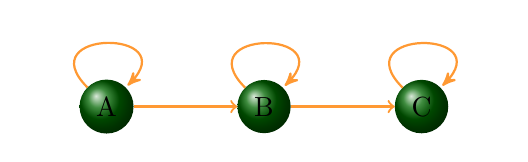
\begin{tikzpicture}
\GraphInit[vstyle=Shade]
\tikzset{EdgeStyle/.style ={->, color = myorange}}
\tikzset{VertexStyle/.style ={shape=circle,ball color = mygreen,}}
\Vertices[unit=2]{line}{A,B,C}
\Edges (A,B,C)
\Loop[dist=30pt, dir=NO](A)
\Loop[dist=30pt, dir=NO](B)
\Loop[dist=30pt, dir=NO](C)
\end{tikzpicture}
\end{center}
\pause
\begin{eqnarray*}
&&f : \{A,B,C\} \to \{0,1\}^2\\
&&f(A) = (0, 0), f(B) = (0,1), f(C) = (1,1)
\end{eqnarray*}
\pause
\[R_1 = \begin{pmatrix}
A & A & B & B & C\\
A & B & B & C & C\\
\end{pmatrix} 
\Rightarrow
R_2 = \begin{pmatrix}
0 & 0 & 0 & 0 & 1 \\
0 & 0 & 1 & 1 & 1 \\
0 & 0 & 0 & 1 & 1 \\
0 & 1 & 1 & 1 & 1 \\
\end{pmatrix} \]
\pause
\[\mathrm{\ccsp(}R_1\mathrm{)}\aple\mathrm{\ccsp(}R_2\mathrm{)}\aple\mathrm{\cbis}\]
\end{example}
\end{frame}

%%%%%%%%%%%%%%%%%%%%%%%%%%%%%%%%%%%%%%%%%%%%%%%%%%%%%%%%%%%%%%%%%%%%%%%%%%%%%%%%%%%%%%%%%%%%%%%%%%%%%%%%%%%%%%%%%%%%%
\section{Reflexive Oriented Graphs}
%%%%%%%%%%%%%%%%%%%%%%%%%%%%%%%%%%%%%%%%%%%%%%%%%%%%%%%%%%%%%%%%%%%%%%%%%%%%%%%%%%%%%%%%%%%%%%%%%%%%%%%%%%%%%%%%%%%%%

%%%%%%%%%%%%%%%%%%%%%%%%%%%%%%%%%%%%%%%
\begin{frame}
\frametitle{Reflexive Oriented Graphs}
\begin{center}
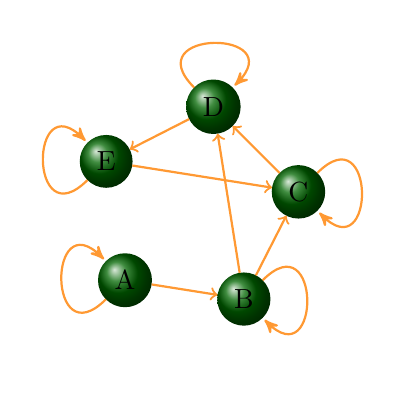
\begin{tikzpicture}
\GraphInit[vstyle=Shade]
\tikzset{EdgeStyle/.style ={->,color = myorange}}
\tikzset{VertexStyle/.style ={shape=circle,ball color = mygreen,}}
\begin{scope}[rotate=-135]
\Vertices[unit=1.3]{circle}{A,B,C,D,E}
\end{scope}
\Edges(A,B,C,D,E)
\Edge (B)(D)
\Edge (E)(C)
\Loop[dist=30pt, dir=WE](A)
\Loop[dist=30pt, dir=EA](B)
\Loop[dist=30pt, dir=EA](C)
\Loop[dist=30pt, dir=NO](D)
\Loop[dist=30pt, dir=WE](E)
\end{tikzpicture}
\end{center}
\pause
\begin{theorem}
If \(H\) is a reflexive oriented graph, 
\[\mathrm{\chom(}H\mathrm{)}\apge \mathrm{\cbis}\]
\end{theorem}
\end{frame}

%%%%%%%%%%%%%%%%%%%%%%%%%%%%%%%%%%%%%%%
\begin{frame}
\frametitle{Notations}
\begin{center}
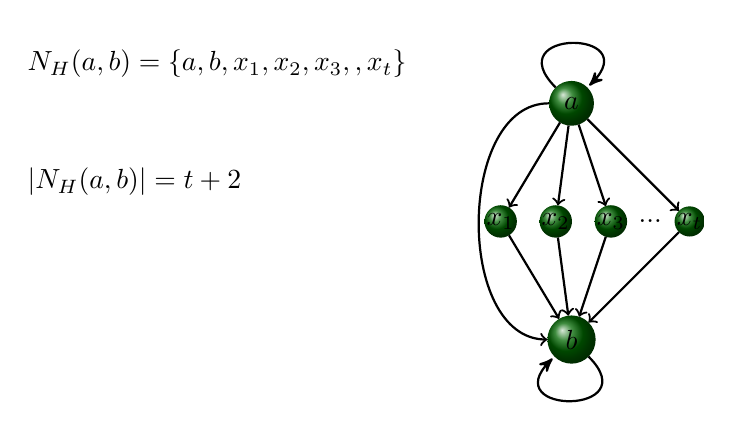
\begin{tikzpicture}
\GraphInit[vstyle=shade]
\node[inner sep=0,anchor=east,text width=5.7cm] (note1) at (0,3.5) {\(N_H(a,b) = \{a, b, x_1, x_2, x_3, \dotsc, x_t\}\)};
\node[inner sep=0,anchor=east,text width=5.7cm] (note2) at (0,2) {\(|N_H(a,b)| = t + 2\)};
\SetVertexMath
\tikzset{VertexStyle/.style ={shape = rectangle}}
\tikzset{VertexStyle/.style ={shape=circle, ball color = mygreen}}
\Vertex[x=1.2, y=3]{a}
\Vertex[x=1.2, y=0]{b}
\tikzset{VertexStyle/.style ={shape=circle, inner sep=0, minimum size=3pt, ball color = mygreen}}
\Vertex[x=0.3, y=1.5]{x_1}
\Vertex[x=1.0, y=1.5]{x_2}
\Vertex[x=1.7, y=1.5]{x_3}
\Vertex[x=2.7, y=1.5]{x_t}
\tikzset{VertexStyle/.style ={shape = rectangle}}
\Vertex[x=2.2, y=1.5]{...}
\tikzset{EdgeStyle/.style ={->}}
\Edge (a)(x_1)
\Edge (a)(x_2)
\Edge (a)(x_3)
\Edge (a)(x_t)
\Edge (x_1)(b)
\Edge (x_2)(b)
\Edge (x_3)(b)
\Edge (x_t)(b)
\Loop[dist=30pt, dir=NO](a)
\Loop[dist=30pt, dir=SO](b)
\tikzset{EdgeStyle/.style ={->, bend right = 90}}
\Edge (a)(b)
\end{tikzpicture}
\end{center}
\pause
\[k(H) = \max_{a\to b}\{|N_H(a,b)|\}\]
\end{frame}

%%%%%%%%%%%%%%%%%%%%%%%%%%%%%%%%%%%%%%%
\begin{frame}
\frametitle{\(k(H)=2\)}
\[k(H) = 2 \Rightarrow N_H(a,b) = \{a, b\}\]
\begin{center}
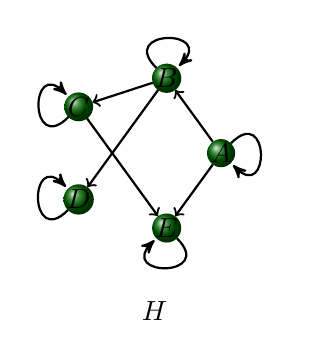
\begin{tikzpicture}
\GraphInit[vstyle=Shade]
\node[inner sep=0,anchor=east,text width=2cm] (note1) at (2,-2) {\(H\)};
\tikzset{VertexStyle/.style ={shape=circle, inner sep=0, minimum size=3pt, ball color = mygreen}}
\SetVertexMath
\Vertices{circle}{A, B, C, D, E}
\tikzset{EdgeStyle/.style ={->}}
\Edges (A, B, D)
\Edge (A)(E)
\Edge (B)(C)
\Edge (C)(E) 
\Loop[dist=20pt,dir=ea](A)
\Loop[dist=20pt,dir=no](B)
\Loop[dist=20pt,dir=we](C)
\Loop[dist=20pt,dir=we](D)
\Loop[dist=20pt,dir=so](E)
\end{tikzpicture}
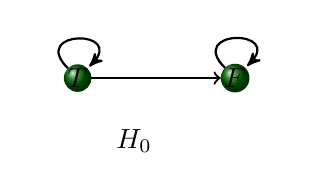
\begin{tikzpicture}
\GraphInit[vstyle=Shade]
\node[inner sep=0,anchor=east,text width=2cm] (note1) at (2.5,-.8) {\(H_0\)};
\tikzset{VertexStyle/.style ={shape=circle, inner sep=0, minimum size=3pt, ball color = mygreen}}
\SetVertexMath
\Vertices[unit=2]{line}{T, F}
\tikzset{EdgeStyle/.style ={->}}
\Edge (T)(F) 
\Loop[dist=20pt,dir=no](T)
\Loop[dist=20pt,dir=no](F)
\end{tikzpicture}
\end{center}
\end{frame}

%%%%%%%%%%%%%%%%%%%%%%%%%%%%%%%%%%%%%%%
\begin{frame}
\frametitle{\(k(H)=2\)}
\[k(H) = 2 \Rightarrow N_H(a,b) = \{a, b\}\]
\begin{center}
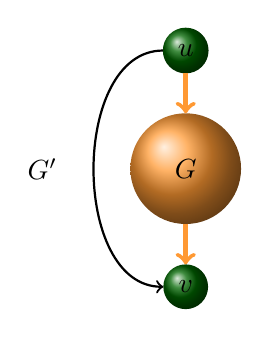
\begin{tikzpicture}
\GraphInit[vstyle=shade]
\SetVertexMath
\node[inner sep=0,anchor=east,text width=2cm] (note1) at (0,1.5) {\(G'\)};
\tikzset{VertexStyle/.style ={shape=circle, ball color = mygreen}}
\Vertex[x=0, y=3]{u}
\tikzset{VertexStyle/.style ={shape=circle, minimum size=40pt, ball color = myorange}}
\Vertex[x=0, y=1.5]{G}
\tikzset{VertexStyle/.style ={shape=circle, ball color = mygreen}}
\Vertex[x=0, y=0]{v}
\tikzset{EdgeStyle/.style ={->, bend right = 90}}
\Edge (u)(v)
\tikzset{EdgeStyle/.style ={->, ultra thick, color=myorange}}
\Edge(u)(G)
\Edge(G)(v)
\end{tikzpicture}
\end{center}
\[\hom(G',H) = |E(H)|.\hom(G,H_0) + |V(H)|\]
\[\mathrm{\chom(}H\mathrm{)} \apge \mathrm{\chom(}H_0\mathrm{)} \apge \mathrm{\cbis}\]
\end{frame}

%%%%%%%%%%%%%%%%%%%%%%%%%%%%%%%%%%%%%%%
\begin{frame}
\frametitle{\(k(H)>2\)}
\begin{center}
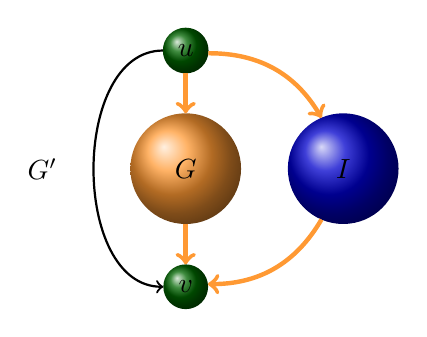
\begin{tikzpicture}
\GraphInit[vstyle=shade]
\SetVertexMath
\node[inner sep=0,anchor=east,text width=2cm] (note1) at (0,1.5) {\(G'\)};
\tikzset{VertexStyle/.style ={shape=circle, ball color = mygreen}}
\Vertex[x=0, y=3]{u}
\tikzset{VertexStyle/.style ={shape=circle, minimum size=40pt, ball color = myorange}}
\Vertex[x=0, y=1.5]{G}
\tikzset{VertexStyle/.style ={shape=circle, minimum size=40pt, ball color = myblue}}
\Vertex[x=2, y=1.5]{I}
\tikzset{VertexStyle/.style ={shape=circle, ball color = mygreen}}
\Vertex[x=0, y=0]{v}
\tikzset{EdgeStyle/.style ={->, bend right = 90}}
\Edge (u)(v)
\tikzset{EdgeStyle/.style ={->, ultra thick, color=myorange}}
\Edge(u)(G)
\Edge(G)(v)
\tikzset{EdgeStyle/.style ={->, ultra thick, color=myorange, bend left}}
\Edge(u)(I)
\Edge(I)(v)
\end{tikzpicture}
\pause
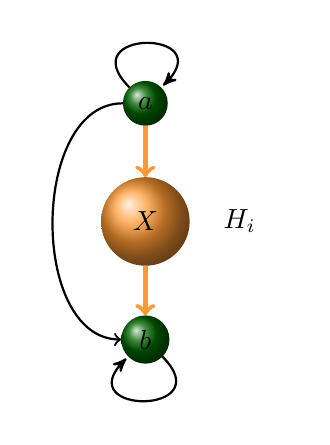
\begin{tikzpicture}
\GraphInit[vstyle=shade]
\node[inner sep=0,anchor=east,text width=1cm] (note1) at (2,1.5) {\(H_i\)};
\SetVertexMath
\tikzset{VertexStyle/.style ={shape = rectangle}}
\tikzset{VertexStyle/.style ={shape=circle, ball color = mygreen}}
\Vertex[x=0, y=3]{a}
\Vertex[x=0, y=0]{b}
\tikzset{VertexStyle/.style ={shape=circle, ball color = myorange, minimum size = 32pt}}
\Vertex[x=0, y=1.5]{X}
\tikzset{EdgeStyle/.style ={->}}
\Loop[dist=30pt, dir=NO](a)
\Loop[dist=30pt, dir=SO](b)
\tikzset{EdgeStyle/.style ={->, ultra thick, color=myorange}}
\Edge (a)(X)
\Edge (X)(b)
\tikzset{EdgeStyle/.style ={->, bend right = 90}}
\Edge (a)(b)
\end{tikzpicture}
\end{center}
\begin{eqnarray*}
&&\mathrm{\chom(}H\mathrm{)} \apge \mathrm{\chom(}H_1 \cup H_2 \cup \dotsb H_t \mathrm{)}\\
&&k(H_i) = k(H)
\end{eqnarray*}
\end{frame}

%%%%%%%%%%%%%%%%%%%%%%%%%%%%%%%%%%%%%%%
\begin{frame}
\frametitle{\(k(H)>2\)}
If all \(H_i\) are isomorphic
\[\hom(G,H) = \hom(G,H_1)^t \Rightarrow \mathrm{\chom(}H\mathrm{)} \apge \mathrm{\chom(}H_1\mathrm{)}\]

By Lov\'asz Theorem \\
If \(H_i\) and \(H_j\) are not isomorphic there exists a graph \(Z\) such that
\[\hom(H_i,Z) \neq \hom(H_j,Z)\]

Without loss of generality assume \(\hom(H_i,Z) > \hom(H_j,Z)\)
\end{frame}

%%%%%%%%%%%%%%%%%%%%%%%%%%%%%%%%%%%%%%%
\begin{frame}
\begin{center}
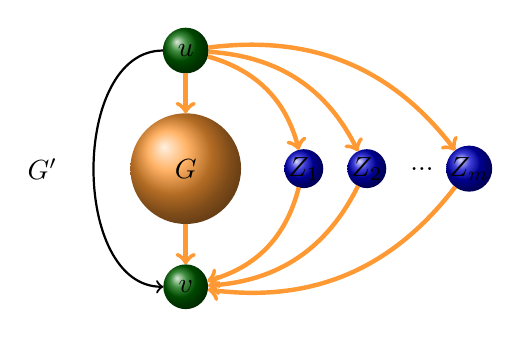
\begin{tikzpicture}
\GraphInit[vstyle=shade]
\SetVertexMath
\node[inner sep=0,anchor=east,text width=2cm] (note1) at (0,1.5) {\(G'\)};
\tikzset{VertexStyle/.style ={shape=circle, ball color = mygreen}}
\Vertex[x=0, y=3]{u}
\tikzset{VertexStyle/.style ={shape=circle, minimum size=40pt, ball color = myorange}}
\Vertex[x=0, y=1.5]{G}
\tikzset{VertexStyle/.style ={shape=circle, ball color = myblue, inner sep=0}}
\Vertex[x=1.5, y=1.5]{Z_1}
\Vertex[x=2.3, y=1.5]{Z_2}
\tikzset{VertexStyle/.style ={shape=rectangle}}
\Vertex[x=3.0, y=1.5]{...}
\tikzset{VertexStyle/.style ={shape=circle, ball color = myblue, inner sep=0}}
\Vertex[x=3.6, y=1.5]{Z_m}
\tikzset{VertexStyle/.style ={shape=circle, ball color = mygreen}}
\Vertex[x=0, y=0]{v}
\tikzset{EdgeStyle/.style ={->, bend right = 90}}
\Edge (u)(v)
\tikzset{EdgeStyle/.style ={->, ultra thick, color=myorange}}
\Edge(u)(G)
\Edge(G)(v)
\tikzset{EdgeStyle/.style ={->, ultra thick, color=myorange, bend left}}
\Edge(u)(Z_1)
\Edge(u)(Z_2)
\Edge(u)(Z_m)
\Edge(Z_1)(v)
\Edge(Z_2)(v)
\Edge(Z_m)(v)
\end{tikzpicture}
\end{center}
\[\mathrm{\chom(}H\mathrm{)} \apge \mathrm{\chom(}H_i\mathrm{)}\]
\end{frame}

%%%%%%%%%%%%%%%%%%%%%%%%%%%%%%%%%%%%%%%
\begin{frame}
\frametitle{\(k(H) > 2\)}
\begin{center}
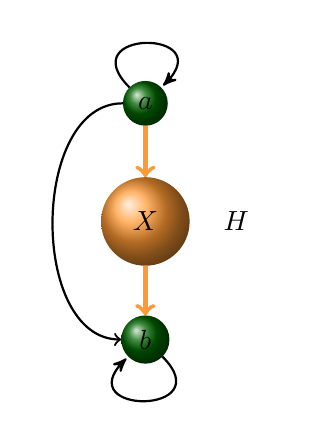
\begin{tikzpicture}
\GraphInit[vstyle=shade]
\node[inner sep=0,anchor=east,text width=1cm] (note1) at (2,1.5) {\(H\)};
\SetVertexMath
\tikzset{VertexStyle/.style ={shape = rectangle}}
\tikzset{VertexStyle/.style ={shape=circle, ball color = mygreen}}
\Vertex[x=0, y=3]{a}
\Vertex[x=0, y=0]{b}
\tikzset{VertexStyle/.style ={shape=circle, ball color = myorange, minimum size = 32pt}}
\Vertex[x=0, y=1.5]{X}
\tikzset{EdgeStyle/.style ={->}}
\Loop[dist=30pt, dir=NO](a)
\Loop[dist=30pt, dir=SO](b)
\tikzset{EdgeStyle/.style ={->, ultra thick, color=myorange}}
\Edge (a)(X)
\Edge (X)(b)
\tikzset{EdgeStyle/.style ={->, bend right = 90}}
\Edge (a)(b)
\end{tikzpicture}
\end{center}
\(d^-(u)\) is minimum in \(H\) by Extended Pinning Lemma
\[\mathrm{\chom(}H\mathrm{)} \apge \mathrm{\chom(}H - u\mathrm{)} \]
\pause
\[2 \le k(H - u) \le k(H) - 1\]
\end{frame}

%%%%%%%%%%%%%%%%%%%%%%%%%%%%%%%%%%%%%%%%%%%%%%%%%%%%%%%%%%%%%%%%%%%%%%%%%%%%%%%%%%%%%%%%%%%%%%%%%%%%%%%%%%%%%%%%%%%%%
\section{Monotone Reflexive Graphs}
%%%%%%%%%%%%%%%%%%%%%%%%%%%%%%%%%%%%%%%%%%%%%%%%%%%%%%%%%%%%%%%%%%%%%%%%%%%%%%%%%%%%%%%%%%%%%%%%%%%%%%%%%%%%%%%%%%%%%

%%%%%%%%%%%%%%%%%%%%%%%%%%%%%%%%%%%%%%%
\begin{frame}
\end{frame}


\end{document}
